\chapter{Reuse}
\label{langchapter}

\section{Introduction}

Languages are hard to design. The effort that goes into producing
a language definition can be overwhelming, particularly if the
language is large or semantically rich. One way to address this
problem is to find ways of designing languages so that they are
more reusable and adaptable. By reusing, rather than re-inventing,
it is possible to significantly reduce the time spent on
development, allowing language designers to concentrate on the
novel features of the language.

This chapter looks at techniques that can be used to design
reusable metamodels. These include approaches based on the use of
specific extension mechanisms such as stereotyping and class
specialisation, and richer mechanisms that support the large
grained extension of modelling languages, such as meta-packages
and package specialisation.  An alternative approach based on the
translation of new concepts into pre-defined is also discussed.

The following sections examine each of these approaches in turn,
identifying their advantages and disadvantages and offering
practical advice on their application.

\section{Extension Based Approaches}
\label{langextension}

This approach involves extending and tailoring concepts from an
existing metamodel. The most common mechanisms for implementing
extension are class specialisation and stereotyping.

\subsection{Specialisation}

Specialisation has been widely used as a reuse mechanism by OO
programming languages for many years. Since XMF is an OO
metamodelling language, it is not surprising that this mechanism
can also be used to reuse language concepts.

One of the best ways to support this approach is to provide a
collection of classes (a framework) that supports a collection of
reusable language concepts. These concepts can then be specialised
to support the new language concepts.

The XCore framework (see section \ref{framework}) aims to support
the abstractions found in popular metamodelling frameworks such as
MOF \cite{mofspec} and EMF \cite{emf} at a usable level of
granularity. An important difference between XCore and other
frameworks is that XCore is a platform independent, executable
language with a precisely defined syntax and semantics. This means
that these semantics can be extended as well to rapidly define
semantically rich language concepts. For example, if the class
XCore::Class is specialised by the class X, all instances of X
will inherit the properties of a class, including the following:

\begin{itemize}
\item They can be instantiated. \item They can have attributes,
operations and constraints. \item They can be serialized. \item
Their instances can be checked against any constraints. \item
Their operations can be invoked on their instances. \item They
have access to the grammar and diagram syntax defined for classes.

\end{itemize}

Furthermore, because the class Class also specialises Object, all
operations that apply to an Object can also be applied to
instances of X, such as executing its meta-operations, mapping it
to another concept and so on.

Having an executable semantics for a metamodelling framework adds
significant value because semantics can be reused along with the
structural properties of the language concepts.

\subsubsection{Example}

Consider the requirement to model the concept of a mapping. A
mapping has the following properties:

\begin{itemize}
\item It has a domain, which is a collection of input types to the
mapping. \item It has a range, which is the result type of the
mapping. \item A mapping can be instantiated and the state of a
mapping instance can be recorded. \item Operations can be defined
on an mapping and can be executed by its instances. \item A
mapping owns a collection of clauses that define patterns for
matching input values to output values. \item A mapping instance
can be executed, matching inputs to clauses and resulting in an
output value.
\end{itemize}

Many of these properties can be reused from existing XCore
concepts, thus avoiding the need to model them from scratch. The
model in figure \ref{mappingspecialisation} shows how this might
be done by specialising the class Class.

\begin{figure}[htb]
\begin{center}
\includegraphics[width=10cm]{LanguageFamilies/figures/mappingspec}
\caption{Reuse of the class Class to define a new Mapping concept}
\label{mappingspecialisation}
\end{center}
\end{figure}

The mapping class reuses all the properties of Class, including
attributes, operations and the machinery to support instantiation
and operation invocation. Other properties, such as having domain
and range types, and executing mappings are layered on top.

\subsection{Stereotyping, Tags and Profiles}
\label{stereotypes}

Stereotypes are a widely used device that enable existing
modelling concepts to be treated as virtual subclasses of an
existing metamodelling class. This is achieved by associating
metamodel classes with information about what stereotypes they may
support. An example of this might be to stereotype the class Class
as a Component and the class Association as a Component Connector.

Tags and tagged values are closely related to stereotypes. These
have the same effect as extending metamodel classes with
additional attributes and information about the values these
attributes may be assigned. An example of tag and tagged value
might be the tag "visibility" attached to an Operation, which can
have the values, "public", "private" or "protected".

Together, stereotypes and tags can be used to create what is
called a {\em profile}: a collection of stereotyped concepts that
form the vocabulary of a new or hybrid modelling language.

Many UML tools provide support for stereotypes, tags and tagged
values, allowing them to be visually displayed in an editor with
an appropriate identifier. Figure \ref{stereotypeExample} shows a
class diagram with two stereotyped classes and a stereotyped
association.

\begin{figure}[htb]
\begin{center}
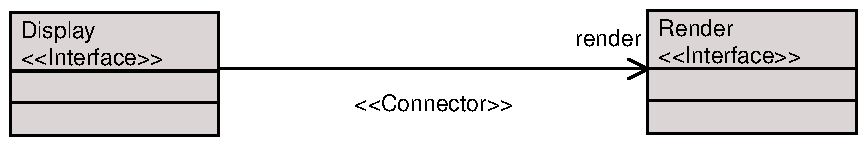
\includegraphics[width=10cm]{LanguageFamilies/figures/Stereotypes}
\caption{Using stereotypes to model interfaces and connectors}
\label{stereotypeExample}
\end{center}
\end{figure}

The advantage of stereotypes and tags is that they add a
convenient level of tailorability to modelling tools that would
otherwise be unavailable.

Nevertheless, stereotypes and tags suffer from being semantically
weak and are not a replacement for a well-defined metamodel of the
language. As the example in figure \ref{wrongstereotypes} shows,
they offer little control over the correct usage of the language:
for instance, a model written in a component modelling language
might not permit interfaces to be connected to classes, yet this
will not be ruled out by stereotypes. Furthermore, stereotypes are
not able to capture the semantics of a language as they cannot
change the properties of meta-classes.

\begin{figure}[htb]
\begin{center}
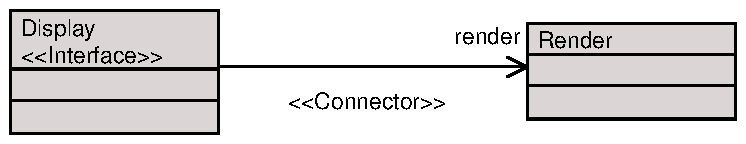
\includegraphics[width=9cm]{LanguageFamilies/figures/WrongStereotypes}
\caption{An example of inconsistencies that can arise through the
use of stereotypes} \label{wrongstereotypes}
\end{center}
\end{figure}

\noindent While UML profiles \cite{umlspec} allow additional
constraints to be defined on stereotypes, there are few if any
tools available that support this capability.

\subsection{Package specialisation and Meta-Packages}
\label{metapackages}

Although specialisation can be used to directly extend metamodel
concepts, this is a significantly more involved process than
defining stereotypes because a concrete syntax for the concepts
will also have to be modelled if they are to be used in a tool. A
better solution would be one that combines the simplicity of
stereotypes with the power of specialisation.

One way of achieving this is through the use of {\em package
specialisation} and {\em meta-packages}. Package specialisation is
a relationship between two packages where the child package
specialises the parent package. The consequence of this is that it
enables a package of language concepts to be clearly identified as
extensions of a package of existing language concepts (the parent
package).

As an example, figure \ref{componentspecialisation} shows a
package of component concepts specialising the XCore package.

\begin{figure}[htb]
\begin{center}
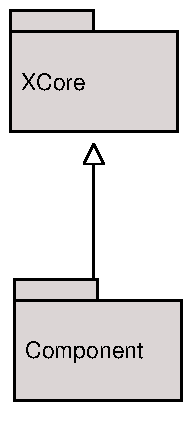
\includegraphics[width=2.5cm]{LanguageFamilies/figures/componentspecialisation}
\caption{Specialising the XCore package}
\label{componentspecialisation}
\end{center}
\end{figure}

Inside the components package some choices are made about the
XCore classes that are to be specialised. These are shown in
figure \ref{componentspecialisation2}. Additional constraints can
be added to rule out certain combinations of components, for
example, a connector must always connect two interfaces.

\begin{figure}[htb]
\begin{center}
\includegraphics[width=10cm]{LanguageFamilies/figures/componentspecialisation2}
\caption{specialising XCore concepts}
\label{componentspecialisation2}
\end{center}
\end{figure}

This provides sufficient information to determine whether a
concept should be represented as a native concrete syntax element
or as a stereotyped element. However, a way must now be found of
{\em using} the specialised package. This is where meta-packages
come in useful. A meta-package is a package of elements that are
instances of elements in another package (the meta-package). In
the components example, a package containing a model written in
the components language is related to the components package by a
meta-package relationship (see figure \ref{metapackage}).

\begin{figure}[htb]
\begin{center}
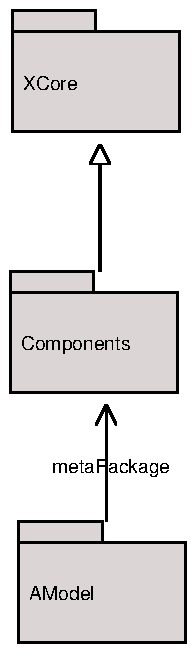
\includegraphics[width=2.5cm]{LanguageFamilies/figures/Metapackage}
\caption{A metapackage relationship between a model and the
components package} \label{metapackage}
\end{center}
\end{figure}

If a tool understands that the model is an instance of a package
that specialises the XCore package it can provide appropriate
stereotypes for each of the specialised elements (see figure
\ref{amodel} for an example). These stereotyped elements can be
used to construct models, which can then be checked against any
constraints in the components package. Because the stereotyped
elements are real instances of meta-model elements all the
semantics inherited from XCore will be available as well.

\begin{figure}[htb]
\begin{center}
\includegraphics[width=10cm]{LanguageFamilies/figures/amodel}
\caption{A model written in the components language}
\label{amodel}
\end{center}
\end{figure}

Meta-packages are a more generic concept than just a mechanism for
dealing with concrete syntax. Consider a language expressed as a
meta-package that already has tools developed for the language. If
a new language differs from the existing one in a few minor but
important ways we would like to make use of the existing tools but
clearly work with the new language. The new language can be
defined as an extension of the meta-package. A package whose
meta-package is the new languages can thus be supplied to the
development tools using the standard principle of substitution.

If tools are generic with respect to the meta-package, then it can
tailor itself by providing specific instances of functionality for
each new language feature that is a sub-class of a corresponding
feature in the meta-package. This may cover a wide range of
different aspects of tool functionality.

As an example, imagine that a configuration management tool
expects instances of any sub-package of XCore and provides
facilities such as rollback, model-merge etc, based on all the
sub-classes of Class, Association, Attribute etc then a wide
variety of development tools can be constructed each of which
works with a different language but which all use the same
development code.

\section{Translation Based Approaches}

The aim here is to define new modelling concepts by a translation
to existing concepts that implement their required properties. As
described in chapter \ref{mappingchapter}, there are a variety of
ways of translating between metamodel concepts. These include:

\begin{itemize}
\item Defining a translation from the concrete syntax of a
concept to an appropriate abstract syntax model written in another
language. The new language is thus a sugar on top of the existing
language.
\item Translating from the abstract syntax of the new concept into
the appropriate abstract syntax model.
\item Maintaining a synchronised mapping between concepts.
\end{itemize}

By translating into an existing primitive, the effort required to
model the semantics of the new concept is significantly reduced.
The translation approach is akin to a compilation step, in which
new concepts are compiled into more primitive, well-defined
concepts. The advantage is that layers of abstraction can be built
up, each ultimately based on a core set of primitives support by a
single virtual machine. This greatly facilitates tool
interoperability as the virtual machine becomes a single point of
tool conformance.

\subsection{Example}

A common approach to implementing associations is to view them as
a pair of attributes and a constraint, where associations between
classes are implemented  as attributes on each class plus a
round-trip constraint that must hold between instances of the
classes. A translation can be defined between an association model
(either expressed as concrete or abstract syntax) and the more
primitive concept of class and attribute.

\section{Family of Languages}
\label{families}

As the number of languages built around a metamodelling language
architecture grows, it is very useful to be able to manage them in
a controlled way. One approach is to organise them into families
of languages \cite{prefaces}. In a family of languages, each
member is related to another language through its relationship to
a common parent. The result is a framework of languages that can
be readily adapted and combined to produce new language members:
in other words a language factory or product line architecture.

There are a number of mechanisms that are useful realising such a
framework. Packages are a good mechanism for dividing languages
into language components, which can be combined using package
import. An example of such an arhictecture is shown in figure
\ref{langarch}.

\begin{figure}[htb]
\begin{center}
\includegraphics[width=8cm]{LanguageFamilies/figures/langarch}
\caption{A language architecture} \label{langarch}
\end{center}
\end{figure}

Packages can be broken down further, both vertically and
horizontally. Vertical decomposition decomposes a language into a
sub-language components that incrementally build on each other. An
example might be an expression language that is arranged into
packages containing different types of expressions: binary, unary
and so on.

A horizontal decomposition breaks a language into different
aspects. It makes sense to make a distinction between the concrete
syntax, abstract syntax and semantic domain of the language
component (see figure \ref{horizontal}).

\begin{figure}[htb]
\begin{center}
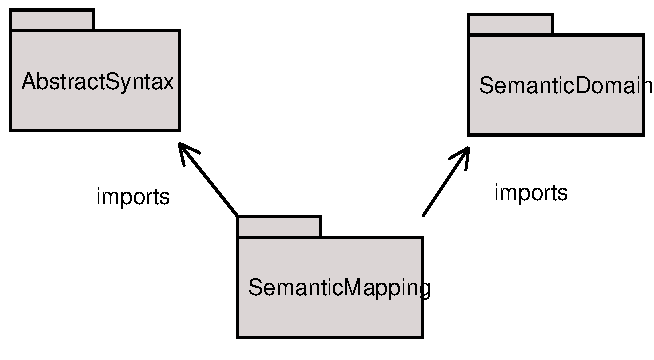
\includegraphics[width=9cm]{LanguageFamilies/figures/horizontal}
\caption{Horizontal language components} \label{horizontal}
\end{center}
\end{figure}

\section{The XCore Framework}
\label{framework}

Figure \ref{xmfframework} shows the class framework for XCore.
This framework is based on a combination of MOF and other
metamodelling frameworks such as Ecore with necessary extensions
to support executability. As such it should be viewed as an
example of a typical metamodelling language framework.

\begin{figure}[htb]
\begin{center}
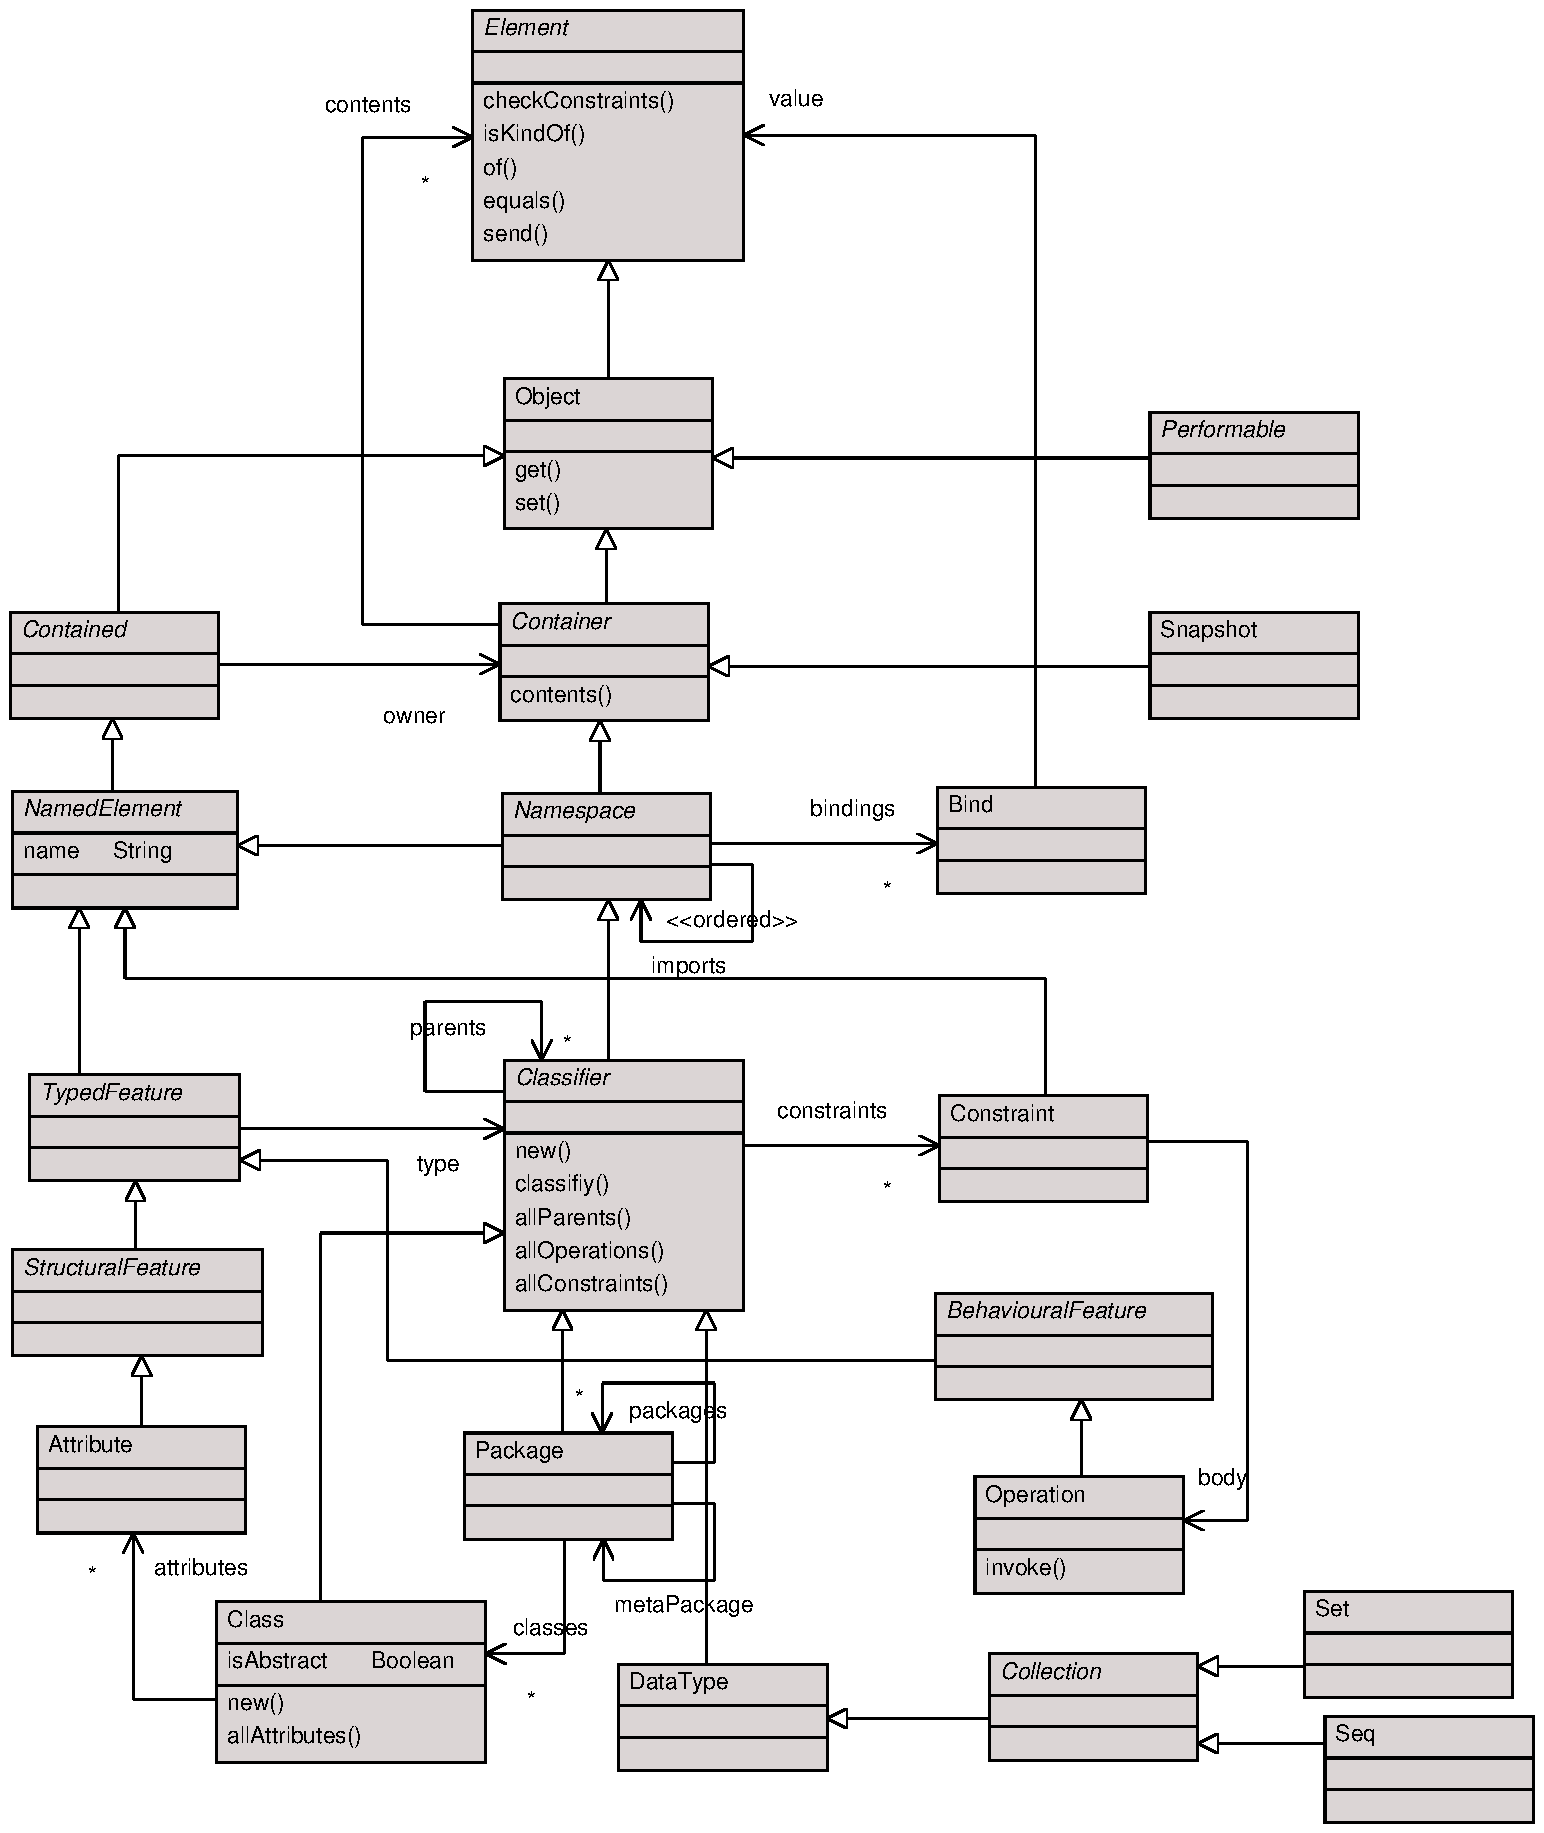
\includegraphics[width=15cm]{XMF/figures/xcore}
\caption{Overview of the XCore class framework}
\label{xmfframework}
\end{center}
\end{figure}

Within this framework there are a number of abstract classes that
encapsulate the generic properties of common types of language
concepts. The following table identifies some of the key ones:

\begin{description}
\item [Classifier] A classifier is a name space for operations and
constraints. A classifier is generalizable and has parents from
which it inherits operations and constraints. A classifier can be
instantiated via new(). In both cases the default behaviour is to
return a default value as an instance. If the classifier is a
datatype then the basic value for the datatype is returned
otherwise 'null' is returned as the default value. Typically you
will not create a Classifier directly, but create a class or an
instance of a sub-class of Class. \item [Container] A container
has a slot 'contents' that is a table. The table maintains the
contained elements indexed by keys. By default the keys for the
elements in the table are the elements themselves, but sub-classes
of container will modify this feature accordingly. Container
provides operations for accessing and managing its contents. \item
[DataType] DataType is a sub-class of Classifier that designates
the non-object classifiers that are basic to the XMF system. An
instance of DataType is a classifier for values (the instances of
the data type). For example Boolean is an instance of DataType -
it classifies the values 'true' and 'false'. For example Integer
is an instance of DataType - it classifies the values 1, 2, etc.
\item [NamedElement] A named element is an owned element with a
name. The name may be a string or a symbol. typically we use
symbols where the lookup of the name needs to be efficient. \item
[Namespace] A name space is a container of named elements. A name
space defines two operations getElement() and hasElement() that
are used to get an element by name and check for an element by
name. Typically a name space will contain different categories of
elements in which case the name space will place the contained
elements in its contents table and in a type specific collection.
For example, a class is a container for operations, attributes and
constraints. Each of these elements are placed in the contents
table for the class and in a slot containing a collection with the
names 'operations', 'attributes'; and 'constraints' respectively.
The special syntax '::' is used to invoke the getElement()
operation on a name space. \item [StructuralFeature] This is an
abstract class that is the super-class of all classes that
describe structural features. For example, Attribute is a
sub-class of StructuralFeature. \item [TypedElement] A typed
element is a named element with an associated type. The type is a
classifier. This is an abstract class and is used (for example) to
define Attribute.

\end{description}

\section{Conclusion}

This chapter has shown the importance of being able to reuse
language definitions rather than having to design new languages
from scratch. Two approaches were presented: specialisation and
translation. specialisation involves reusing pre-existing language
concepts via class specialisation. A framework of language
concepts is important for this purpose. The advantage of the
approach is that it enables tools to rapidly adapt their
functionality to support new concepts. Translation involves
mapping new concepts to existing concepts. It is particularly
useful when constructing layered definitions in which richer
abstractions are translated down onto more primitive abstractions.
